%
% to embed text in math, use \mbox:
%
%  $S \mbox{ where } x \in S \implies \mbox{$x$~is full of fish heads}$
%
%


\documentclass[11pt,twoside]{article}
\usepackage{natbib}
\usepackage{amssymb}
\usepackage{amsmath}
\usepackage{amsthm}
\usepackage[letterpaper,inner=1.375in, outer=1.125in, top=1.25in, bottom=1in]{geometry}
\usepackage{graphicx}
\usepackage{setspace}
\usepackage{array}
\usepackage{tabularx}
\usepackage{verbatim}

\newcommand\dnr{\ensuremath{\mathit{DNR}}}
\newcommand\fail{\mathit{FAIL}}
\newcommand\pass{\mathit{PASS}}
\newcommand\defined{\mathrel{\;\stackrel{\scriptscriptstyle\mathbf{def}}{=}\;}}


\newtheorem{thm}{Theorem}
\theoremstyle{definition}
\newtheorem{defn}{Definition}

\let\cite=\citep
\bibpunct();A{},




\begin{document}

\advance\extrarowheight by 1.5pt

\title{Finding the Signal: Improved Ranking and Noise Reduction in Black Box Testing}
\author{Jesse Welch}
\date{May 2012}

\pagestyle{headings}


\maketitle

\begin{abstract}
We present algorithms for analyzing multiple programs that solve the
same problem.  The algorithms help an analyst rank the programs and
diagnose each program's faults.

We rank programs objectively by analyzing the results of black-box
testing.  Our analysis encompasses a richer notion of "result" than
that used in prior work.  And our method can analyze incomplete
results, which enables us to run more tests faster by batching tests.

We also use black-box test results to help diagnose a program's
faults.  Naive diagnostics list all tests a program failed.  Prior
work presents only the failures necessary to rank programs---a shorter
list.  By discovering relationships between tests, our algorithm
presents an even shorter, less noisy diagnostic list.
\end{abstract}

\newpage
\tableofcontents
\newpage

\baselineskip=1.2\baselineskip % a little extra space between lines


\section{Introduction}
When a professor receives a submissions of student homework assignments, there are two tasks they face: grading the assignments, and providing the students with useful feedback. Without an algorithmic approach, these tasks are extremely daunting. Reading the source code of dozens of students, grading their quality, and providing feedback that gives insights into what went wrong is an unpleasant task at best, and an untenable one at worst.

Ideally, we want to find a total ordering of the quality of the students' work, so that grading is trivial. We also want to a list of every bug in a student's program, as short as possible. And we want to do this with a minimum of effort.

Our issues in grading imply a more general problem: given multiple programs solving the same problem, how do we compare them, and how do we diagnose their faults, with a minimum of expert intervention? The first step in the process is to utilize black-box testing, to avoid having to read source code.

But these black-box test results still do not achieve our goals. We do not have a way of creating a fair ordering of the solution's quality. Until a suitable algorithm was proposed, ranking still needed to be done on the basis of expert knowledge. Prior work has descirbed an algorithm for this purpose. In this paper, we present a new method for simplifying the ranking produced, and several methods for increasing its power.

Once solutions are ranked, we still need to find a way to diagnose their faults. Naively, we can simply present the result of every test the solution fails, but this output will certainly not be as possible. Prior work has demonstrated a method for minimizing this list. In this paper, we present a novel method for minimizing the number of failures presented.

\section{Ranking Solutions}
\subsection{What is Ranking?}

The problem of ranking multiple solutions can be simplified to a simpler subproblem. Given two solutions to the same problem, how do we rank their correctness? Claessen et. al. \cite{Claessen} described a fundamental truth for comparing two solutions. Solution $S_1$ is superior to solution $S_2$ if it can solve every problem $S_2$ can, and at least one more.

Ranking algorithms must respect this rule. Even simple algorithms, such as ranking on raw percentage of tests passed, still correctly rank solutions to which this rule applies. 

However, naive algorithms, such as raw percentage, introduce more relationships into the ranking that are not defined by this rule. If two solutions are incomparable based on this rule, because each is able to solve a problem the other is not, they will still be ranked by raw percentage.

We define a ``good'' ranking algorithm as one which ranks based on this rule alone, and does not have additional relationships caused by accidents in the data. A ranking can be improved by removing relationships caused by data accidents, and moving closer to a ranking defined entirely by this rule.

\subsection{A Good Ranking Algorithm}
Claessen et. al. demonstrated an algorithm for creating a fair ranking of solutions\cite{Claessen}. Their algorithm was run on large test suites generated automatically using QuickCheck \cite{QuickCheck}, which produces many similar test cases. Some of these tests will introduce new information, but many of them will test parts of the program already covered by already tests. Rather than considering each test, they considered each piece of information provided by a test. They did this by partitioning the test set into equivalene classes. 

\begin{defn}[Test Equivalence]
Given tests $T_0$ and $T_1$ and solution set $S$
$$ T_0 \equiv T_1 \defined \forall s \in S : s(T_0) \equiv s(T_1) $$
\end{defn}


Using this example, a test set $T$ could be reduced into a set of its equivalence classes. From these equivalence classes, a single representative example could be drawn, creating a new test set $T'$. $T'$ is a simpler set to work with than $T$, and processing it will be cheaper due to its decreased size. Most importantly, because $T'$ contains a representative for every piece of information introduced in $T$, the reduction has not lost any information.

%TODO: Proof by contradiction of this

Claessen's algorithm then creates a partial order of the solutions using $T'$. It does this using a binary representation of results. Tests can either be passed or failed, and PASS $>$ FAIL.

\begin{defn}[Rank order of solutions]
Solution comparisons create a partial order. If neither of these definitions apply, they are incomparable.
Given solutions $S_1$ and $S_2$, and test set $T$, we define
$$S_1 \equiv S_2 \defined \forall t \in T : S_1(t) = S_2(t)$$
$$S_1 \sqsubseteq S_2 \defined \forall t \in T' : S_1(t) \leq S_2(t)$$
When $S_1 \sqsubseteq S_2$ but $S_1 \not\equiv S_2$, we write
$S_1 \sqsubset S_2$.
\end{defn}
Under this definition, there are 4 possible results for comparing two solutions, $S_1$~and~$S_2$. 
$S_1 \sqsubset S_2$, $S_1 \sqsupset S_2$, $S_1 \equiv S_2$, or $S_1$ and $S_2$  are incomparable. This definition allows us to build a partial ordering. This ranking is not built on the number of failures, but only on the direct relationships between the set of tests failed by each solution.

Using this algorithm, we are able to successfully create fair rankings of different student solutions. Figure 1 demonstrates one such ranking.

\begin{figure}
\centering
\includegraphics{rank1.ps}
\caption{An edge points from a functionally inferior solution to a functionally superior one. "$\vert$" represents a class of tests passed by the equivalence class, "." represents a class of tests failed by the equivalence class.}
\end{figure}

\subsection{More Tests are Always Better}
When we build a test suite, we don't want to build it by carefully crafting tests that explore each edge case. Like ranking solutions and providing witnesses, we want the expert running the test set to have to spend as little time as possible creating the test set. Ideally, they could automatically generate thousands of tests, and the algorithm would find the relevant information. Property-based testing plans, such as QuickCheck \cite{QuickCheck} follow this concept, as does any other form of automatic test generation.

The title of the section is a slight overstatement. To be precise, more tests are never worse. If we have a test set with 0 tests, it will rank every solution as identical. If we add one test, this single equivalence class may be retained, or it may break into two classes with an edge between them. A second test can leave the structure unchanged, break one or both of the equivalence classes into two, or remove the edge between them. Each test that we add can break equivalence classes into 2 classes or remove edges, both a form of information gain.

%TODO: Add a 3 step figure showing every possible way the classes can be laid out. Use a dotted arrow to represent a relationship that may or may not exist.

\begin{thm} Adding a test to the test set can never cause a loss of information.
\end{thm}

\subsection{Real Problems Have Many Outcomes}
The Claessen algorithm is based upon property-based testing, for which the only possible outcomes are PASS and FAIL. Other forms of testing produce more outcomes. For example, a solution can produce the right output, produce the wrong output, throw an exception, have a fatal error, or fail to terminate in a reasonable amount of time, among other possible outcomes.

Claessen's definitions already allow for more than binary outcomes. We need not change anything except what $>$ means. This step, however, presents an interesting problem. When allowing only binary outcomes, the total order of outcomes is self-evident: PASS$>$FAIL. When dealing with non-binary outcomes, however, there is no readily available ordering. Is an error that crashes the process ``better'' than one that silently produces wrong answers? In some cases, the process should be kept running at all costs. In others, the increased visibility of a catastrophic failure may be preferred to the subtle incorrectness of a wrong answer. In truth, the ranking of these outcomes is an arbitrary decision.

Since no universally correct ordering of outcomes is possible, we chose to examine what would happen if the algorithm was extended by a ordering determined by arbitrary choice. Though many orders could have been tried, for experimental purposes, we imposed a single simple arbitrary order on our three possible outcomes: PASS, FAILURE, and FATAL ERROR : PASS$>$FAILURE$>$FATAL ERROR. We chose this ordering because our datasets represent student solutions, and the students were told that a segmentation fault (or related fatal error) would result in a 0\% as their grade on functional correctness.


\begin{figure}
\centering
\includegraphics[scale=0.75]{rank1.ps}
\caption{Created using binary outcomes}
\includegraphics[scale=0.75]{rank2.ps}
\caption{Created using multiple outcomes}
\end{figure}

Using our new comparison function (but an algorithm unaltered from Claessen's), we an interesting properties. As demonstrated in Figures 2 and 3, in many cases, the additional outcome made no difference. In these cases, not only did solutions in the same equivalence class fail the same test, they failed them in the same way.

In a small subset of our test cases
%TODO: quantify
we were able to improve the ranking using multiple outcomes. In most of these cases, it rendered incomparable solutions previously considered equivalent. This was due to them failing on the same tests, but in varying ways. In rare cases, we were able to rank solutions previously considered equivalent, generally because the solutions were identical, except on a subset of test on which one segfaulted and the other produced invalid output.

\subsection{The Cost of Testing Matters}

The computational power required to test a program adequately can be substantial. To fully exercise a medium-scale program, over a thousand unit tests may be required (in our data, as many as 2468 tests were run on each solution). Additionally, we tested some programs where testing would take over an hour per solution, distributed across the lab cluster.

The number of tests required is frequently too large to affordably run sequentially. In an experimental test infrastructure, we attempted to testing this code sequentially, spawning two processes per test (one for the solution, and one for the reference implementation). Testing in this manner took ~4 hours of CPU time. When the tests were instead batch processed, with one process being spawned per group of related tests, testing took ~1.5 minutes of CPU time.

Large tests also present a difficult issue. Distributed testing has its own set of problems, and when running these large tests, something may go wrong, causing the test to "randomly" fail. These tests are simply too expensive to run repeatedly in an attempt to get a result.

Because of the high cost of testing, we must use batch testing and allow large tests to fail to complete. These solutions introduce a new problem: what do we do with the lack of test results? If a test does not run on a particular solution, we shouldn't throw out the results on the remaining solutions. This would destroy data successfully gathered. Instead, we introduce a new test result, which is achieved implicitly by any solution on a test for which it does not report a result: Did Not Run (\dnr). Note that \dnr means specifically that a test was not run at all. An outcome such as Did Not Finish (DNF) would appear explicitly in the test set.

With these new outcomes ``in'' our dataset, we were faced with the challenge of ranking based on them. There were two possible paths for ranking these solutions. The first would be to simply use the process described in the previous section, and extend the comparison function to place DNR arbitrarily within the ordering (perhaps as the worst result, or equivalent to a fatal error). This solution is simple, and allows us to reuse the modifications above. However, by giving \dnr a place in the ordering, we define its value in a way that may not be true. If a test does not run due to the fatal error in an earlier test during batching, \dnr would have a negative meaning. But if a large, distributed test fails, it is for effectively arbtirary reasons. Giving \dnr a meaning in this case would be creating information about the solution, which may or may not be true.

To avoid inventing information, we can choose another method for handling \dnr outcomes. The procedure is very simple.
\begin{defn}[Rank order with \dnr]
Given solutions $S_1$ and $S_2$, and test set $T$, we define
$$S_1 \equiv S_2 \defined \forall t \in T : S_1(t) \neq \dnr \wedge S_2(t) \neq \dnr : S_1(t) \equiv S_2(t)$$
$$S_1 > S_2 \defined \forall t \in T : S_1(t) \neq \dnr \wedge S_2(t) \neq \dnr : S_1(t) \geq S_2(t)$$
\end{defn}
In this way, we do not invalidate any of the possible meanings of \dnr. If the \dnr is caused by a failure in batch testing, the test whose failure caused it to not run still has a result in the data set. Under the above definitions, we will compare based on this test, and still be able to create a ranking that is true to the data. If the \dnr happened for an arbitrary reason, such as a failure in the testing infrastructure, by ignoring it, we do not introduce meaning to the test. 

Using this process, solutions can be compared whenever tests are not run, for whatever reason they are not run. If tests are not run for a reason, we can still compare the solutions, based solely on the reason, \emph{without information loss}.

\section{Finding Relationships Between Tests}
\subsection{Some Outcomes Imply Other Outcomes}
The methods described above treat each test as distinct. Tests are used to compare solutions, but they are never compared to each other, and they are treated as if they were independent. In real test sets, there are frequently subset of the tests which are not independent.

An example of this occurred when we tested student solutions to the problem of reducing terms in the lambda calculus. These reductions are the result of a sequence of deterministic steps in which (most) lambda calculus terms are reduced to their simplest form, using $\beta$- and $\eta$-reductions. One feature we tested was whether students had properly implemented $\eta$-reduction. To properly perform $\eta$-reductions, the student code should reduce any term of the form $\lambda a.M_\eta a$ to $M_\eta$, whereever it occurs, as long as $a$ is not free in $M_\eta$. To test this, we enumerated terms with "holes" in them, and placed an $\eta$-redex within the hole. Two terms created are: 
$$T_1 : \lambda a.M_\eta a
T_2 : \lambda x.\lambda x.\lambda a.M_\eta a$$
$T_1$ tests an $\eta$-reduction on its own, with no other variables. These terms were all generated automaticlly, but viewing the terms generated, we hypothesized that, if a student was to correctly reduce any other terms containing $\eta$-reductions, such as $T_2$, they would need to be able to successfully reduce $T_1$.
If our hypothesis is correct, there should be an underlying relationship in the data set. Failing $T_1$ should imply failing $T_2$. Additionally, failing $T_1$ should imply failing every other test that contains an $\eta$-reduction.

This is only one example of a potential implication. Datasets contain many more such relationships. We have classified these relationships into four categories:
\begin{itemize}
\item \emph{Real Implications}---implications such as $T_1 \Rightarrow T_2$ above, which document an actual relationship between tests. 
\item \emph{Accidental Implications}---implications which are represented in the data, but have no bearing on the outer world, and are instead an "accident" of the solution population. 
\item \emph{Trivial Implications}---tautological implications, which are true regardless of the data set. 
\item \emph{Bogus Implications}---implications which are defined within the data, but which, given a sufficiently large population of solutions, could not possibly exist.
\end{itemize}

%We create a structure we call the implication graph, which documents these implications. The simple implication graph includes every implication from all four classes. An improved implication graph attempts to eliminate as many trivial, bogus, and accidental implications as possible, while retaining the real implications.

\subsection{The Naive Set of Implications}
\begin{defn}[Outcome Implication]
Given solution set $S$ and outcomes $O_1$ on test $T_1$ and $O_2$ on test $T_2$
$$O_1 \Rightarrow O_2 \defined \forall s \in S : s(T_1) = O_1 : s(T_2) = O_2$$
\end{defn}

Using this definition, we discover every observed implication in the dataset, the union of every representative of every class of implications defined above. First we create a proposition for every outcome, and its inverse, on every test. Then we look for an implication (in either direction) between each pair of propositions. This is a $O(n^2)$ process, but by limiting computation to one test from each equivalence class of tests, $n$ remains small enough to proceed (in our experiences, $n$ is between 6 and 144).

This process is simplified by usage of a variation of the partitioning algorithm used to create the equivalence classes of tests. Rather than partitioning the tests, we partition the \emph{propositions} into equivalence classes. For a given solution, a proposition is considered true if it holds on that solution (e.g. the proposition Test 2 PASS hold for a solution if it passes Test 2), and false if it does not hold. Two propositions, $P_1$ and $P_2$, are considered equivalent if they hold for the exact same set of solutions.
$$P_1 \equiv P_2 \defined \forall s \in S : P_1(s) = P_2(s)$$
Now, rather than having to find implications between every proposition, we need to find them between every \emph{class} of propositions.

The set of implications within a dataset forms a natural structure: a directed graph. Each class of propositions is a node in the graph, and each implication is an edge from the implicating proposition to the implied. An example of a naive implication graph appears in Figure 4.

\begin{figure}
\verbatiminput{toyimpldata}
\includegraphics[width=\textwidth]{toyimpl.ps}
\caption{Dataset and the generated implication graph. A transitive reduction has been performed on the graph}
\end{figure}

Given this implication graph, the question remains: How many of the implications in the graph are real implications? We were provided with a natural experiment to begin to test this question. Our students were given an assignment that contained 14 problems. Each of the problems was entirely self-contained, and there was no code overlap between the problems. Some problems covered related topics, and so relic relationships might appear in the data, but by and large, we expected these problems to be diagrammed as entirely separate components.

\begin{figure}
\includegraphics[width=\textwidth]{div.ps}
\caption{Implication graph generated from experiment. Subproblems form subcomponents, but no subcomponent is separated from the rest of the graph}
\end{figure}

\begin{comment}
\begin{figure}
\includegraphics[width=0.45\textwidth,bb=200 100 300 150,clip=true]{div.ps}
\includegraphics[width=0.45\textwidth,bb=300 150 500 350,clip=true]{div.ps}
\caption{Implication graph generated from experiment. Boxed sections indicate tests performed on the same problem. TODO: ADD BOXES}
\end{figure}
\end{comment}



The results of this experiment were mixed. We did not find that every subproblem made an entirely separate subgraph, but instead that the subproblems made subgraphs that were sometimes connected, with implications between portions of the problem that should not be possible in the underlying problem.

\subsection{Improving the Implication Graph}

The implication graph contains every implication of all four classes (real, accidental, trivial, and bogus). An ideal graph contains every real implication, and no other implications. Creating this graph is not possible, even in principle, but there are several methods for limiting or eliminating the members of the negative three classes.

First, we can readily remove two types of bogus implications. An implication is bogus if it exists in the implication graph, but could not exist given a sufficient population of solutions. The two types of implications we can remove are any implications of the form $\pass\Rightarrow\fail$ or $\fail\Rightarrow\pass$.

Assumption: There exists a fully correct and fully incorrect solution to every problem.


\begin{thm} $\pass(T_1)$ cannot imply $\fail(T_2)$

\begin{proof} Assume $\pass(T_1) \Rightarrow \fail(T_2)$. This means that every solution that passes $T_1$ fails $T_2$. However, there exists the fully correct solution S. For all tests T, S(T) = PASS. Therefore S($T_1$) = PASS, and S($T_2$) = PASS, contradicting our assumption.
\end{proof}
\end{thm}

\begin{thm} $\fail(T_2)$ cannot imply $\pass(T_1)$

\begin{proof} Assume $\fail(T_1) \Rightarrow \pass(T_2)$. This means that every solution that fails $T_1$ passess $T_2$. However, there exists the fully incorrect solution S'. For all tests T, S'(T) = FAIL. Therefore S'($T_1$) = FAIL, and S'($T_2$) = FAIL, contradicting our assumption.
\end{proof}
\end{thm}



Based on these proofs, we can safely remove from the implication graph every implication between the passage of one test and the failure of another. This can be done in one of two ways. Either we can look for the implication graph and remove these implications where they exist, or we can create it with a fully correct and a fully incorrect solution as members of the solution set.

Introducing the fully correct and fully incorrect solutions will also remove a class of trivial implications: implications created from tests with uniform outcomes. If every solution gets the same outcome on a given test, this outcome will be trivially implied by every outcome of every test. Similarly, if no student gets an outcome on a given test, this outcome trivially implies every outcome of every test. These implications add no useful information, and can either be removed explicitly, or implicitly by the introduction of the fully correct and incorrect solutions.

There is a related type of accidental implication we can remove, though this one must be removed explicitly. If a particular outcome is achieved by exactly one equivalence class of solutions, this outcome will trivially imply every other outcome achieved by this class. If solution $S$ is the only solution to fail test $T_1$, and also fails $T_2$ and $T_3$, $\fail(T_1) \Rightarrow \fail(T_2)$ and $\fail(T_1) \Rightarrow \fail(T_3)$ regardless of the outcomes of every other solutions. This is because every solution that failed $T_1$ (only S) also achieved every other outcome S achieved. 

Removing this set of implications is particularly important, because they are highly misleading. They make the claim that, if you know one thing about a solution, you can know everything about it, which is untrue. They are not classified as bogus, however, because the implication may actually be real. We simply don't have enough information to know.

We can also easily remove another type of trivial implication: tautologies. A tautology exists when an implication will hold true regardless of the dataset, for example : $\pass(T_1) \Rightarrow \neg\dnr(T_1)$ and $\dnr(T_1) \Rightarrow \neg\fail(T_1)$. These implications can simply be removed, because they do not add any useful information to the set of implications.

These reductions are able to improve the ratio between real implications and the other classes, but they are not perfect. Notably, we do not have a way to differentiate between real and accidental implications. We believe there may exist more heuristics to remove further implications, particularly accidental implications.

\section{Noise Reduction}

\subsection{What is Noise?}
A piece of data is classified as noise if it can be removed without causing any loss of information. For example, in Table 1 (below) we show that the number of tests run is generally far greater than the number of equivalence classes they form. However, for our ranking algorithm, we only need a single representative from each equivalence class to create our ranking. The non-representative members of each equivalence class are noise. 

As described above, our goals include creating an accurate ranking of programs, and providing a solution's creator with a minimum subset of failed tests, to diagnose faults as easily as possible. Noise reduction on the ranking does not improve (or reduce) its accuracy, but it does make the ranking graph simpler to read and interpret. Nosie reduction on the witness set provided to a solution directly achieves our stated goal, minimizing the amount of information provided.


\subsection{Claessen's Algorithm}
Claessen's paper on ranking describes are several forms of noise reduction. The first is the fundamental step of the algorithm, in which tests are grouped into equivalence classes. This step alone reduces from the original number of tests to a substantially smaller subset (see Table 1 below).

After this large-scale reduction, Claessen's algorithm contains another form of noise reduction. 

\begin{defn}[Claessen Redundancy]
A test $T_0$ is redundant if
$$\fail (T_0) \equiv \fail(T_1) \cup \fail(T_2)$$
\end{defn}
where all three tests are drawn from different equivalence classes. This definition was justified with the argument that, rather than discovering a new faults of its own, $T_0$ likely provoked both of the faults discovered in $T_1$ and $T_2$. Removing $T_0$ therefore does not cause any information loss. Instead, its removal simplifies the test set to a smaller, but still representative sample of tests.

\subsection{Union*}
The logical basis to Claessen's algorithm that a test can be redundant because it provokes the flaws already demonstrated by two other non-redundant tests\cite{Claessen}, can be extended further. Why should we limit this to only circumstances where the flaws are in exactly two other tests? Why not any number? We propose an extended algorithm, one which removes any tests whose set of failures is equal to the union of the failures of \emph{any number of tests}. 

\begin{defn}[Union* Redundancy]
A test $T_0$ is redundant if

$$\fail (T_0) \equiv \fail(T_1) \cup \fail(T_2) \cup ... \cup \fail(T_n) $$
\end{defn}

The implication graph allows us to create a simple implementation of this algorithm. First we find the node which contains the failure of test $T_0$. By looking at the in-edges, we can easily find the subset of tests $T'$ whose failures imply $T_0$. $T_0$ is redundant if $\fail(T_0) \equiv \cup^* T'$.

\subsection{Comparison}
Union* must reduce at least as many tests as Claessen, and can reduce more. This is because every test that will be removed under Claessen will be removed under exactly the same conditions in Union* (the union of two tests is simply a specification of the union of any number of tests). In theory, Union* is capable of outperforming Claessen

\begin{figure}
\verbatiminput{testset}
\includegraphics{toy.ps}
\caption{Reduced under Claessen. t = {1,2,3,4}}
\includegraphics{toyb.ps}
\caption{Reduced under Union*. t = {1,2,3}}
\end{figure}

%TODO: Table with different levels of reductions. Then change the text below to handle whatever I put in the table.

In practice, results were mixed. Out of 21 datasets tests, Claessen and Union* performed identically 18 times. In the 3 datasets reduced, it reduced an average of 3 tests per test set, a 5\% reduction.

\begin{table}[t]
\def\?{\phantom0}
\centering

\begin{tabular}{ | l | c | c | c | c | }
\hline
        &          &             &   After   & After \\ 
Dataset & \#~Tests & \#\ Classes &  Claessen &  Union*  \\ 
     &            &             & Reduction & Reduction \\
\hline
105 & \?135 & \?\?8 & \?8 & \?8 \\
all & \?\?20 & \?10 & \?8 & \?8 \\
asm & \?\?96 & \?27 & 19 & 18 \\
asmcoding & \?135 & \?\?6 & \?5 & \?5 \\
bitpack & 2468 & 144 & 91 & 87 \\
comp40intro & \?\?20 & \?12 & 10 & 10 \\
divtest & 2112 & \?71 & 40 & 40 \\
eq & \?\?\?6 & \?\?4 & \?4 & \?4 \\
extras & \?\?45 & \?\?9 & \?7 & \?7 \\
inf & \?\?96 & \?71 & 46 & 42 \\
linterp & \?435 & \?31 & 20 & 20 \\
nr & \?\?22 & \?10 & 10 & 10 \\
pred & \?\?\?6 & \?\?3 & \?3 & \?3 \\
required & \?\?54 & \?11 & \?9 & \?9 \\
size & \?180 & \?26 & 19 & 19 \\
sudoku & \?19 & \?\?6 & \?6 & \?6 \\
tuscheme & \?\?96 & \?49 & 38 & 38 \\
typesys & \?\?85 & \?41 & 33 & 33 \\
u & \?256 & \?53 & 29 & 29 \\
unblack & \?23 & \?14 & 14 & 14 \\
unify & \?256 & \?53 & 29 & 29 \\
\hline
\end{tabular}
\caption{The results of each reduction algorithm}
\end{table}

There are several hypotheses for the fact that Claessen and Union* generally perform identically. One is that no test tests more than two underlying faults. This is extremely unlikely, as it is relatively simple to write a test that exercises large sections of a program's functionality, and can readily provoke more than two potential faults. Another possibility lies in the method of building tests. When unit tests are written, they generally exercise small areas of functionality, rather than the entire program. A different style of test design might allow Union* to have more success, removing large tests that attempt to exercise every possible fault in the program, when these faults are better demonstrated by small tests. A final possibility is that we simply don't have enough solutions, and that a greater diversity in solutions would increase the difference between the two algorithms.




\section{Reducing Noise in Witness Sets}
\subsection{Witness Sets}
As described above, when grading students, successfully ranking them is not the only goal of creating and running a test set. An additional goal is providing the student with feedback on the flaws within their program. We do this programmatically by creating a "witness set", a list of every test the solution has failed, and a witness documenting what went wrong.

This witness set is drawn only from the tests which are used to rank the student solutions. Thus, the noise-reduction strategies above implicitly reduce noise in the witness set, by eliminating tests from consideration. However, this still leaves many tests in the witness set, and we observe many which appear similar or redundant. If this noise can be reduced, students can be provided a simpler set of witnesses, making it easier for them to understand the flaws in their programs.

\subsection{The Algorithm}
We have already performed a large amount of witness reduction using the algorithms above. After creating equivalence classes, and applying Union*, we need only report a single result from each remaining witness class. However, there are still redundancies in the witness set. By performing a further reduction, on a single solution rather than the solution set as a whole, we can reduce further. When looking at a single solution, only one type of relevant relationship remains: the relationships between tests.

The implication graph is a representation of the relationships between these tests. It presents many discoverable relationships (implies, implied by, reachable from, etc.). Using this graph, we are able to perform noise reduction at the level of a single solution, a novel process. For simplicity, we chose to examine only one of the available relationships, direct implication. Our algorithm is as follows:

\begin{defn}[Witness Set Reduction]
Solution $S$ has naive witness set $W$, where $W$ is the set of all tests $T$ where $S(T) = \fail$.
Reduced witness set $W'$ is the largest subset of $W$ such that
$$\forall T_1, T_2 \in W' : T_1 \not\Rightarrow T_2$$
\end{defn}

As an algorithm, this is implemented by removing witnesses from the naive witness set.
\begin{defn}[Witness Reduction Algorithm]
Given witness set $W$, we remove test $T_0$ if
$$\exists T_1 \in W : T_1 \Rightarrow T_0$$
\end{defn}

Given a perfect implication graph, in which every implication is not just found in the data but representative of the problem itself, this algorithm reduces the tests presented as  failed to the set of the easiest tests failed. 

If two tests are needed to differentiate the solutions on the solution class scale, it is possible (and frequently true), that one is simply an easier version of itself. For example, take the lambda terms described above when creating the implication graph. 

$$T_1 : \lambda a.M_\eta a$$
$$T_2 : \lambda x.\lambda x.\lambda a.M_\eta a$$

The data confirmed our hypothesis that a flaw in $T_1$ caused a failure in $T_2$. The implication graph contained the implication $\fail(T_1) \Rightarrow \fail(T_2)$. This led our algorithm to be able to reduce the witnesses to any solution who failed both tests, providing only the output from $T_1$.

\begin{figure}
\verbatiminput{lambdareduction}
\caption{Machine output for a successful reduction in which $T_2$ (nr403) was removed due to failure of $T_1$ (nr97)}
\end{figure}

\subsection{Validity of Reductions}

This witness reduction algorithm successfully reduces witness sets. But these reductions are based on an implication graph which is imperfect by definition. This led us to the hypothesis that many of the reductions performed might appear to have been performed based on accidental implications, and are therefore not good reductions to have made.

To test this, we carried out an experiment. We used a data set also used above for the purpose of validating the implication graph. This data set represented a homework problem in which students were asked to write 14 different functions. In the reference implementation, all of these functions were entirely independent, and not call any of the other assigned functions. Based on this fact, we chose to define an accidental implication as any implication between tests of different functions, and a real implication as any implication between tests on the same function.

\begin{comment}
\begin{figure}
\verbatiminput{goodreductions}
\caption{Valid reductions.}
\verbatiminput{badreductions}
\caption{Invalid reductions.}
\end{figure}

\begin{figure}
\verbatiminput{example.witness}
\caption{Unreduced output}
\verbatiminput{example3.witness}
\caption{Reduced with unreduced implication graph}
\verbatiminput{example2.witness}
\caption{Reduced using improved implication graph}
\caption{In the student's code, none of the subproblemss call each other. Therefore any implication between subproblems was accidental based on the code base.}
\end{figure}
\end{comment}

%\begin{figure*}
%\begin{tabularx}{\linewidth}{@{}XX@{}}
%\small\verbatiminput{goodreductions}
%&
%\small\verbatiminput{badreductions}
%\\
%\caption{Good reductions}&
%\caption{Bad reductions}
%\\
%\end{tabularx}
%\end{figure*}

When we ran this experiment using the naive implication graph, we found that 447 reductions were performed. Of these, 264 were deemed to be based on valid implications, an accuracy of 59.1\%. When we ran it with the reduced implication graph, there were only 422 reductions. Of these, the same 264 were deemed to be based on valid implications, an accuracy of 62.5\%. This moderately low accuracy was in large part due to a large number of accidental implications involving some of the least correct solutions. When the two least correct solutions were removed from the data set, only 350 reductions were performed, 260 of which were deemed valid, an accuracy of 74.3\%.

\begin{comment}
\begin{figure}
\verbatiminput{example.witness}
\caption{Unreduced output}
\verbatiminput{example3.witness}
\caption{Reduced with unreduced implication graph}
\verbatiminput{example2.witness}
\caption{Reduced using improved implication graph}
\caption{In the student's code, none of the functions call each other. Therefore the reduction across tests is not only invalid under our metric, but accidental based on the code base.}
\end{figure}
\end{comment}

\section{Future Work}
\subsection{Witness Expansion}

In this paper, we use the implication graph to remove noisy information from the witness set. However, the implication graph may potentially be usable to \emph{create} information, providing more accurate diagnostic information by \emph{expanding} the witness set. 

When we believed two tests were related based on the implication graph, we removed the more complex test, because the simpler one provided the diagnostic information. However, for a more successful solution, which passed the simple test but failed the complex one, we provide no evidence of this relationship. But this relationship clarifies where the fault lies. Using a very similar formula to our witness reduction, we can provide the student with these relationships.

\centerline{We inform a solution $S$ which passed test $T_1$ but failed $T_2$ of the results on  $T_1$ iff}
$$ S(T_1) = PASS \wedge S(T_2) = \fail \wedge \fail(T_1) \Rightarrow \fail(T_2)$$

\subsection{Additional Reduction Algorithms on the Ranking Graph}

We have only implemented a reduction algorithm based on the union of failure sets. Additional algorithms are certainly possible, and potentially more successful. Potential future algorithms include removing tests if they are the intersection of other failure sets, or if their results are entirely implied by other tests.

\section{Conclusion}
When presented with a large number of solutions to the same problem, we want to be able to rank them on their quality and witness their faults. We want both this ranking and witness set to be minimal, and to be generated with a minimum of human intervention.

Already in the literature are algorithms to rank programs based on black-box testing results. These algorithms are successful, but we have extended the algorithms to take advantage of more available information. Our extended algorithms are capable of refining the ranking by using every result state produced by a natural set of test cases. Additionally, they can process incomplete result sets, allowing testing to be performed more cheaply.

We have also implemented several forms of noise-reduction, to create simpler rankings and witness sets. To reduce rankings, we have introduced the Union* algorithm, a generalization of the reduction strategy implemented in \cite{Claessen}. In practice, this algorithm proved to only occasionally reduce more tests than the base algorithm. However, it \emph{is} capable of reducing more tests, and \emph{is not} capable of reducing less tests.

Our witness reduction algorithm is an entirely novel form of noise reduction. Beyond the reductions performed in reducing the ranking, which work on the entire solution set, our algorithm is able to further reduce witnesses by analyzing each solution individually.

\bibliographystyle{plainnat}
\bibliography{thesis}

\end{document}
